\documentclass{article}

% if you need to pass options to natbib, use, e.g.:
%     \PassOptionsToPackage{numbers, compress}{natbib}
% before loading neurips_2020

% ready for submission
% \usepackage{neurips_2020}

% to compile a preprint version, e.g., for submission to arXiv, add add the
% [preprint] option:
%     \usepackage[preprint]{neurips_2020}

% to compile a camera-ready version, add the [final] option, e.g.:
%     \usepackage[final]{neurips_2020}

% to avoid loading the natbib package, add option nonatbib:
\usepackage[final]{neurips_2020_ml4ps}

\usepackage[utf8]{inputenc}
\usepackage[T1]{fontenc}
\usepackage{hyperref}
\usepackage{url}
\usepackage{float}
\usepackage{booktabs}
\usepackage{amsfonts}
\usepackage{nicefrac}
\usepackage{microtype}
\usepackage{acronym}
\usepackage{amsfonts}
\usepackage{amsmath}
\usepackage{amssymb}
\usepackage{amsthm}
\usepackage{wrapfig}
\usepackage{booktabs}
\usepackage{color}
\usepackage{enumitem}
\usepackage{fontawesome}
\usepackage{natbib}
\usepackage{pgfplots}
\usepackage{siunitx}
\usepackage{tikz}
\usepackage{rotating}
\usepackage{xspace}

\usetikzlibrary{arrows.meta}
\usetikzlibrary{shapes.arrows}
\usetikzlibrary{calc}

\setcitestyle{numbers,square,sort&compress}

\newcommand{\gl}[1]{{\color{blue}{\{#1\}}}}
\newcommand{\todo}[1]{{\color{red}{\it\noindent TODO: #1}}}

\newcommand{\animicon}{{\color{xlinkcolor}\faPlayCircle}\xspace}
\newcommand{\nbicon}{{\color{xlinkcolor}\faFileCodeO}\xspace}

%\newcommand{\acronym}[1]{{\small{#1}}\xspace}
\newcommand{\package}[1]{\textsl{#1}\xspace}
\newcommand{\Euclid}{\textsl{Euclid}\xspace}
\newcommand{\lcdm}{$\Lambda$CDM\xspace}
\newcommand{\kpc}{\textrm{kpc}}
\newcommand{\Msun}{\textrm{M}_\odot}
\newcommand{\kmps}{\textrm{km\,s}^{-1}}
\newcommand{\zl}{z_l}
\newcommand{\zs}{z_s}
\newcommand{\sv}{\sigma_v}
\newcommand{\mtwo}{m_{200}}
\newcommand{\MMW}{M_\textrm{MW}}
\newcommand{\Mtwo}{M_{200}}
\newcommand{\ctwo}{c_{200}}
\newcommand{\rtwo}{r_{200}}
\newcommand{\Rtwo}{R_{200}}
\newcommand{\gdone}{$\textsc{gd-}\oldstylenums{1}$}
\newcommand{\tage}{$t_\text{age}$}
\newcommand{\palfive}{Pal 5}

\newcommand{\eg}{{e.\,g.}\xspace}
\newcommand{\ie}{{i.\,e.}\xspace}
\newcommand{\diff}{\mathrm{d}}
\newcommand{\overbar}[1]{\mkern 1.5mu\overline{\mkern-1.5mu#1\mkern-1.5mu}\mkern 1.5mu}
\newcommand{\fsub}{f_{\mathrm{sub}}}
\newcommand{\nsub}{n_{\mathrm{sub}}}
\newcommand{\pref}{p_{\mathrm{ref}}}
\newcommand{\stattheta}{\ensuremath{\vartheta}\xspace}
\newcommand{\mean}[1]{\makebox[0pt]{$\phantom{#1}\overline{\phantom{#1}}$}#1}

\DeclareMathOperator*{\argmin}{arg\,min}
\DeclareMathOperator{\pois}{Pois}
\DeclareMathOperator{\uniform}{Uniform}
\DeclareMathOperator{\normal}{\mathcal{N}\!}
\DeclareMathOperator{\expectation}{\mathbb{E}}
\DeclareMathOperator{\cov}{cov}
\DeclareMathOperator{\var}{var}
\DeclareMathOperator*{\argmax}{arg\,max}

% Inline code annotation
\newcommand{\code}[1]{\href{#1}{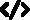
\includegraphics[scale=0.8,trim=0 0.05cm 0 0]{figures/code}}}

% Acronyms
\newacro{BH}[BH]{black hole}
\newacro{GW}[GW]{gravitational wave}
\newacro{PSD}[PSD]{noise power spectral density}

% Supervision and discussion.
\newcommand{\glnote}[1]{\textcolor{red}{[GL]: #1}}
\newcommand{\jhnote}[1]{\textcolor{blue}{[JH]: #1}}
\newcommand{\gbnote}[1]{\textcolor{black}{[GB]: #1}}
\newcommand{\cwnote}[1]{\textcolor{green}{[CW]: #1}}
\newcommand{\NB}[1]{\textcolor{red}{[NB]: #1}}
\newcommand{\CW}[1]{\textbf{(\color{red} CW: #1)}}

\newcommand{\cw}[1]{\textbf{\color{red}[CW: #1]}}


\title{Probing Dark Matter Substructure with Stellar Streams and Neural Simulation-Based Inference}

\author{
  Joeri Hermans \\
  University of Li{\`e}ge \\
  \texttt{joeri.hermans@doct.uliege.be} \\
  \And
  Nilanjan Banik \\
  Texas A\&M University \\
  \texttt{banik@tamu.edu} \\
  \And
  Christoph Weniger \\
  University of Amsterdam \\
  \texttt{c.weniger@uva.nl} \\
  \And
  Gianfranco Bertone \\
  University of Amsterdam \\
  \texttt{g.bertone@uva.nl} \\
  \And
  Gilles Louppe \\
  University of Li{\`e}ge \\
  \texttt{g.louppe@uliege.be}
}

\begin{document}

\maketitle

\begin{abstract}
  This work applies recent advances in simulation-based inference to probe dark matter substructures in the Milky Way halo.
  By simulating the stellar density variations caused by subhalo impacts on stellar streams, and tying those to the WDM thermal relic mass,
  the technique allows us to efficiently compute preliminary, and statistically diagnosed constraints on the dark matter particle mass.  Using existing GD-1 data, we find that the proposed approach has to potential to constrain the WDM mass above 15 keV, provided that simulator systematics can be controlled.
\end{abstract}

\section{Introduction and cosmological context}
\label{sec:introduction}
Cold Dark Matter (CDM) models~\citep{1982ApJ...263L...1P,1984Natur.311..517B} predict
a hierarchical collapse in which large haloes form through the merging of smaller dark matter clumps~\cite{moore1999dark,avila1998formation,zhao2003growth}.
This process is driven by CDM's scale-free halo mass function~\cite{hofmann2001damping,schneider2013halo} and depends 
on the initial conditions of the matter power spectrum, which in turn 
anticipates the existence of 
dark matter haloes down to $10^{-4}~\Msun$ (solar masses)~\cite{bertschinger2006effects}.
Warm Dark Matter (WDM) models~\cite{bond1983collisionless,dodelson1994sterile,2001ApJ...556...93B} on the other hand, in which the dark matter particle is much lighter, influence
structure formation down to the scale of dwarf galaxies. While at large scales the collapse in WDM is hierarchical as well, it becomes strongly suppressed
below $10^9~\Msun$, where the non-negligible velocity dispersion of dark matter particles prevents haloes to form and smooths the density field instead~\cite{smith2011testing}.
The discrepancies between CDM and WDM at these smaller scales provide a powerful test bed to examine the nature of the dark matter particle.
Perturbations in the stellar density of cold globular cluster %stellar
streams~\cite{banik2018probing,banik2019novel,Bonaca:2020psc,bonaca2019spur,bovy2016shape,Banik:2018pal} caused by gravitational interactions with (small-scale) dark matter substructure~\cite{ibata2002uncovering,johnston2002lumpy,yoon2011clumpy,carlberg2012dark}
in the Milky Way halo make
streams an ideal probe to characterize the dark matter particle. However, such perturbations are also attributable to
interactions with baryonic structures in our Galaxy, such as the bar, spiral arms and the galactic population of the Giant Molecular Clouds. It is therefore crucial to study stream systems sufficiently distant
from these baryonic structures, such as GD-1, to confidently detect subhalo impacts~\cite{banik2019effects}.

While forward modeling these complex interactions is relatively straightforward,
the simulation model does not easily lend itself to statistical inference;
the computation of the likelihood involves solving an
intractable inverse problem which rests on the integration of all stochastic execution paths implicitly defined by computer code.
Despite the intractability,
it remains however possible to infer the underlying probabilities by relying on
likelihood-free approximations. This approach is generally referred
to as \emph{likelihood-free}
or \emph{simulation-based} inference~\citep{cranmer2020frontier}.
Previous analyses~\cite{banik2018probing,banik2019novel} relied Approximate Bayesian Computation (ABC)~\citep{rubin1984bayesianly}
to constrain the thermal relic mass of the dark matter particle by \emph{manually} crafting
a summary statistic based on the (partial) power spectrum of a streams stellar density variations.
However, ABC is \emph{only} exact whenever the summary statistic
is \emph{sufficient} and the distance
function chosen to express the similarity between
observed and simulated data tends to 0, which in practice is never achievable.
This work proposes to solve the \emph{intractability} of the likelihood by
learning an amortized mapping
from target or model parameters $\vartheta$ and observables $x$ to posterior densities by solving a
\emph{tractable} minimization problem. The learned mapping has the potential
to increase the statistical power of an analysis since the procedure
\emph{automatically} learns an internal representation of the data.
To support the reproducability of this work,
we provide all code\footnote{\href{https://github.com/JoeriHermans/constraining-dark-matter-with-stellar-streams-and-ml}{\texttt{github.com/JoeriHermans/constraining-dark-matter-with-stellar-streams-and-ml}}}.
Every result is annotated with~\code{https://github.com/JoeriHermans/constraining-dark-matter-with-stellar-streams-and-ml}, which links to the code used to generate it.

\section{Posterior inference through density ratio estimation}
\label{sec:method}
In this work we jointly infer {\bf target parameters} $\vartheta$ which include the WDM
thermal relic mass $m_\textsc{wdm}$ and the stream age \tage.
Given the Bayesian perspective of this analysis, we define the priors over the WDM mass $m_\text{wdm}$ and stream age \tage~as
$\texttt{uniform}(1,~50)$ keV and $\texttt{uniform}(3,~7)$ billion years (Gyr) respectively.
The upper bound corresponds to a half-mode mass of $\sim 4 \times 10^4~\Msun$,
whereas the prior over the stream age is based on the stream length and width.  The length
of the stream and the associated velocity dispersion indicate a stream age of at least 3.4 Gyr~\citep{webb2019searching}.
However, the width of some regions in GD-1 are quite thin, which is
indicative of a low velocity dispersion. A possible explanation for this is that
the stream is in fact older, but that the thicker regions are formed by encounters
with dark matter or baryonic structures. Following this argument, and using the
stream thickness of the thinnest regions, the upper limit is
estimated to be about 7 Gyr~\citep{banik2019novel}.
{\bf Observables $x$} encapsulate the (normalized) stellar density of mock streams --- produced by the
simulation or forward model --- and the \emph{observed} GD-1 normalized stellar density.
\begin{figure*}
    \centering
    \resizebox{\linewidth}{110pt}{
    \begin{tikzpicture}[align=center]
        % BEGIN NEURAL NETWORK -------------------------
        % Container
        \draw [rounded corners, thick] (-2,2) rectangle (2,-2);
         % Draw arrow to log ratio
        \draw [black!100, -Latex] (2 - 0.6667, 2 - 0.6667) -- (2 + 0.6667, 2 - 1 * 0.6667);
        % Draw lines between input and hidden
        \foreach \in in {2,...,4}
            \foreach \hidden in {1,...,5}
                \draw [black!20] (-2 + 1 * 0.667, 2 - \in * 0.6667) -- (0, 2 - \hidden * 0.6667);
        % Draw lines between hidden and log ratio
        \foreach \hidden in {1,...,5}
            \draw [black!20] (0, 2 - \hidden * 0.6667) -- (2 - 0.6667, 2 - 0.6667);
        % Input layer
        %\draw [fill=lightgray!10, draw=gray!100] (-2 + 1 * 0.6667, 2 - 1 * 0.6667) circle [radius=0.25];
        \draw [fill=lightgray!10, draw=gray!100] (-2 + 1 * 0.6667, 2 - 2 * 0.6667) circle [radius=0.25];
        \draw [fill=lightgray!10, draw=gray!90] (-2 + 1 * 0.6667, 2 - 3 * 0.6667) circle [radius=0.25];
        \draw [fill=lightgray!10, draw=gray!90] (-2 + 1 * 0.6667, 2 - 4 * 0.6667) circle [radius=0.25];
        \draw [fill=lightgray!10, draw=gray!90] (0, 2 - 1 * 0.6667) circle [radius=0.25];
        \draw [fill=lightgray!10, draw=gray!90] (0, 2 - 2 * 0.6667) circle [radius=0.25];
        \draw [fill=lightgray!10, draw=gray!90] (0, 2 - 3 * 0.6667) circle [radius=0.25];
        \draw [fill=lightgray!10, draw=gray!90] (0, 2 - 4 * 0.6667) circle [radius=0.25];
        \draw [fill=lightgray!10, draw=gray!90] (0, 2 - 5 * 0.6667) circle [radius=0.25];
        % Output layer (log ratio)
        \draw [fill=lightgray!10, draw=gray!90] (2 - 0.6667, 2 - 1 * 0.6667) circle [radius=0.25];
        % END NEURAL NETWORK ---------------------------
        % Draw the log-ratio
        \node [rounded corners, draw, thick, minimum height=0.9cm, minimum width=2cm, shape=rectangle, anchor=west] (log_ratio) at (2 + 0.6667, 2 - 0.6667) {$\log \hat{r}(x\vert\vartheta)$};
        \node [rounded corners, draw, thick, minimum height=0.9cm, minimum width=2cm, shape=rectangle, anchor=west] (log_prior) at (2 + 0.6667, -2 + 0.6667) {$\log p(\vartheta)$};
        \node [rounded corners, draw, thick, minimum height=0.9cm, minimum width=1.5cm, shape=rectangle, anchor=east, right of=log_ratio, xshift=4cm] (discriminator) {$d(\vartheta,x)$};
        \path let \p1 = (log_ratio) in node [draw,fill=white,thick,circle,below of=log_ratio,above of=log_prior] (plus) at (\x1, 0) {+};
        \draw [black!100, -Latex] (log_ratio) -- ++(discriminator) node[midway,fill=white] {$\sigma(\log\hat{r}(x\vert\vartheta))$};
        \draw [black!100, -Latex] (log_ratio) -- ++(plus);
        \draw [black!100, -Latex] (log_prior) -- ++(plus);
        % Make the axes
        \draw [thick, -Latex] (5.5, -2 + 0.3) -- (10.5, -2 + 0.3) node[anchor=north, yshift=-0.5cm, xshift=-0.25cm] {$m_\textsc{wdm}$};
        \foreach \x in {1,10,20,30,40,50}
            \draw (5.5 + \x / 11, -2 + 0.3 - 0.1) -- (5.5 + \x / 11, -2 + 0.3 + 0.05) node[anchor=north, yshift=-0.15cm] {$\x$};
        % Draw the PDF
        \draw [thick, line width=0.75mm] (5.6, -2 + 0.3) .. controls (6, -0) and (6, -1.4) .. (10.05, - 2 + 0.3);
        \path let \p1 = (plus) in node [rounded corners, draw, minimum height=0.9cm, thick, minimum width=2cm, shape=rectangle, anchor=west] (pdf) at (4.5, \y1) {$\log \hat{p}(\vartheta\vert x)$};
        \draw [-Latex] (plus) -- (pdf);
        \path let \p1 = (pdf) in node [fill=none, opacity=1] (corner) at (9.75, \y1) {};
        \draw (pdf) -- (corner.center) node[midway,fill=white] {$\exp(\log\hat{p}(\vartheta\vert x))$};
        \node [opacity=1] (intersect) at (9.75, -2 + 0.2) {};
        \draw [-Latex] (corner.center) -- (intersect);
        % Draw theta line
        \draw (9.75, -2 + 0.3) -- (9.75, -2 - 0.6);
        \draw (9.75, -2 - 0.6) -- (-2 - 2 * 0.6667, -2 - 0.6);
        \path let \p1 = (log_prior) in node [-Latex, fill=white] (log_prior_bottom) at (\x1, -2 - 0.6) {$\vartheta$};
        \draw [-Latex] (log_prior_bottom) -- (log_prior);
        \draw (-2 - 2 * 0.6667, -2 - 0.6) -- (-2 - 2 * 0.6667, 0 - 0.667);
        \draw [-Latex] (-2 - 2 * 0.6667, 0 - 0.667) -- (-2, 0 - 0.6667);
        \node [fill=white] (inputs) at (-2 - 0.6667, 0 - 0.6667) {$\vartheta$};
        % Draw outputs stuff
        \draw [-Latex] (-2 - 3 * 0.6667, 0 + 0.6667) -- (-2, 0.6667);
        \node [fill=white] (outputs) at (-2 - 0.6667, 0 + 0.6667) {$x$};
        \node[inner sep=0pt] (stream) at (-2 - 4.5 * 0.6667, 0.6667) {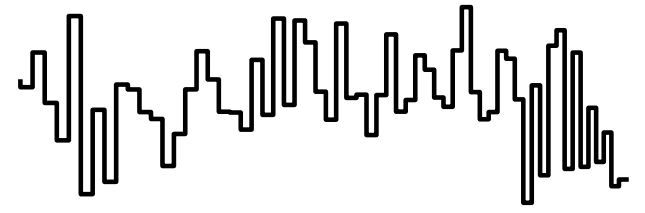
\includegraphics[width=3.5cm]{figures/stream-tikz.png}};
        \node (stream_label) at (-2 - 4.5 * 0.6667, 2 * 0.75) {Observed stellar density};
    \end{tikzpicture}
    }
    \caption{Graphical representation of the inference procedure after training the ratio estimator (neural network).
    The ratio estimator accepts a target parameter $\vartheta$ and an observable $x$ as inputs,
    which are subsequently used to approximate the likelihood-to-evidence ratio $\hat{r}(x\vert\vartheta)$.
    The discriminator output $d(\vartheta, x)$ --- the sigmoidal projection $\sigma(\cdot)$ of $\log\hat{r}(x\vert\vartheta)$ --- is only used during training.}
    \label{fig:overview}
\end{figure*}

The Bayesian paradigm finds model parameters compatible with observation by
computing the \emph{posterior} $p(\vartheta\vert x)$.
Evaluating Bayes' rule in our setting is not possible as the
likelihood $p(x\vert\vartheta)$ is per definition intractable.
To enable the tractable evaluation
of the posterior, we have to rely on likelihood-free surrogates
for key components in Bayes' rule. Note that Bayes' rule can be factorized into
the product of the tractable prior probability and the
likelihood-to-evidence ratio $r(x\vert\vartheta)$:
\begin{equation}
    p(\vartheta\vert x) = p(\vartheta)\frac{p(x\vert\vartheta)}{p(x)} = p(\vartheta)\frac{p(\vartheta,x)}{p(\vartheta)p(x)} = p(\vartheta)r(x\vert\vartheta).
\end{equation}
\citet{2019arXiv190304057H} show that an amortized estimator $\hat{r}(x\vert\vartheta)$
of the intractable likelihood-to-evidence ratio can be obtained
by training a discriminator $d(\vartheta, x)$ with inputs $\vartheta$ and $x$, to distinguish between samples from the
joint $p(\vartheta, x)$ with class label 1 and samples from the product of marginals $p(\vartheta)p(x)$ with class label 0 using a discriminative criterion such
as the binary cross entropy.
Whenever the training criterion is minimized, the authors theoretically
demonstrate that the optimal discriminator $d(\vartheta, x)$
models the Bayes-optimal decision function
\begin{equation}
  d(\vartheta, x) = \frac{p(\vartheta, x)}{p(\vartheta,x) + p(\vartheta)p(x)}.
\end{equation}
Subsequently, given a model parameter $\vartheta$ and an observable $x$,
we can use the discriminator as a density \emph{ratio estimator}
to compute the likelihood-to-evidence ratio
\begin{equation}
  r(x\vert\vartheta) = \frac{1 - d(\vartheta,x)}{d(\vartheta,x)} = \frac{p(\vartheta, x)}{p(\vartheta)p(x)} = \frac{p(x\vert\vartheta)}{p(x)} .
\end{equation}
%However, the computation of this formulation suffers from significant numerical issues
%in the saturating regime where the output of the discriminator tends
%to 0. Considering that $\log r(x\vert\vartheta) = \text{logit}(d(\vartheta, x))$ for classifiers
%with a \emph{sigmoidal} projection at the output, it is possible to directly obtain
%$\log r(x\vert\vartheta)$ from the classifier
%by extracting the quantity before the sigmoidal operation.
%This strategy ensures that the approximation of $\log r(\vartheta\vert x)$
%is numerically stable. 
The posterior probability density can be approximated for arbitrary $\vartheta$ and $x$ by computing $\log p(\vartheta\vert x) \approx \log p(\vartheta) + \log \hat{r}(x\vert\vartheta)$,
%\begin{equation}
%  \log p(\vartheta\vert x) \approx \log p(\vartheta) + \log \hat{r}(x\vert\vartheta),
%\end{equation}
provided that $\vartheta$ and $x$ are supported
by the product of marginals $p(\vartheta)p(x)$.
The ratio estimator can likewise be used to compute a credible region (\textsc{cr}) at a desired level of uncertainty $\alpha$
by constructing a region $\Theta$ which satisfies
$\label{eq:credible_interval}\int_\Theta p(\vartheta)r(x\vert\vartheta)~d\vartheta = 1 - \alpha.$
Since many such regions $\Theta$ exist, we select the
highest posterior density region, which is the smallest \textsc{cr}.

\section{Experiments and results}
\label{sec:results}
\noindent{\bf Simulations}~~10 million pairs $(\vartheta,x)\sim p(\vartheta,x)$ are drawn from the simulation model for training, and
100,000 for testing. The simulations in the training dataset are reused in our \textsc{abc} analyses.

\noindent{\bf Ratio estimator training}~~
The ratio estimators
use \textsc{selu}~\citep{selu} activations and were trained using the \textsc{adamw}~\citep{adamw} optimizer for 50 epochs
with a batch-size of 4096. We found that larger batch-sizes, for our setting, generalized better.
This work considers a \textsc{resnet-50}~\citep{resnet} architecture with
1 dimensional convolutions without dilations.
Because our methodology treats $\vartheta$ as an input feature, we cannot easily
condition the convolutional layers of the \textsc{resnet}-based architectures on $\vartheta$.
This would require conditional convolutions~\citep{yang2019condconv} or hypernetworks~\citep{ha2016hypernetworks} to generate specialized kernels for a given $\vartheta$.
To retain the simplicity of our architecture, we inject the dependency on
$\vartheta$ in the fully connected trunk.
\begin{figure*}
    \centering
    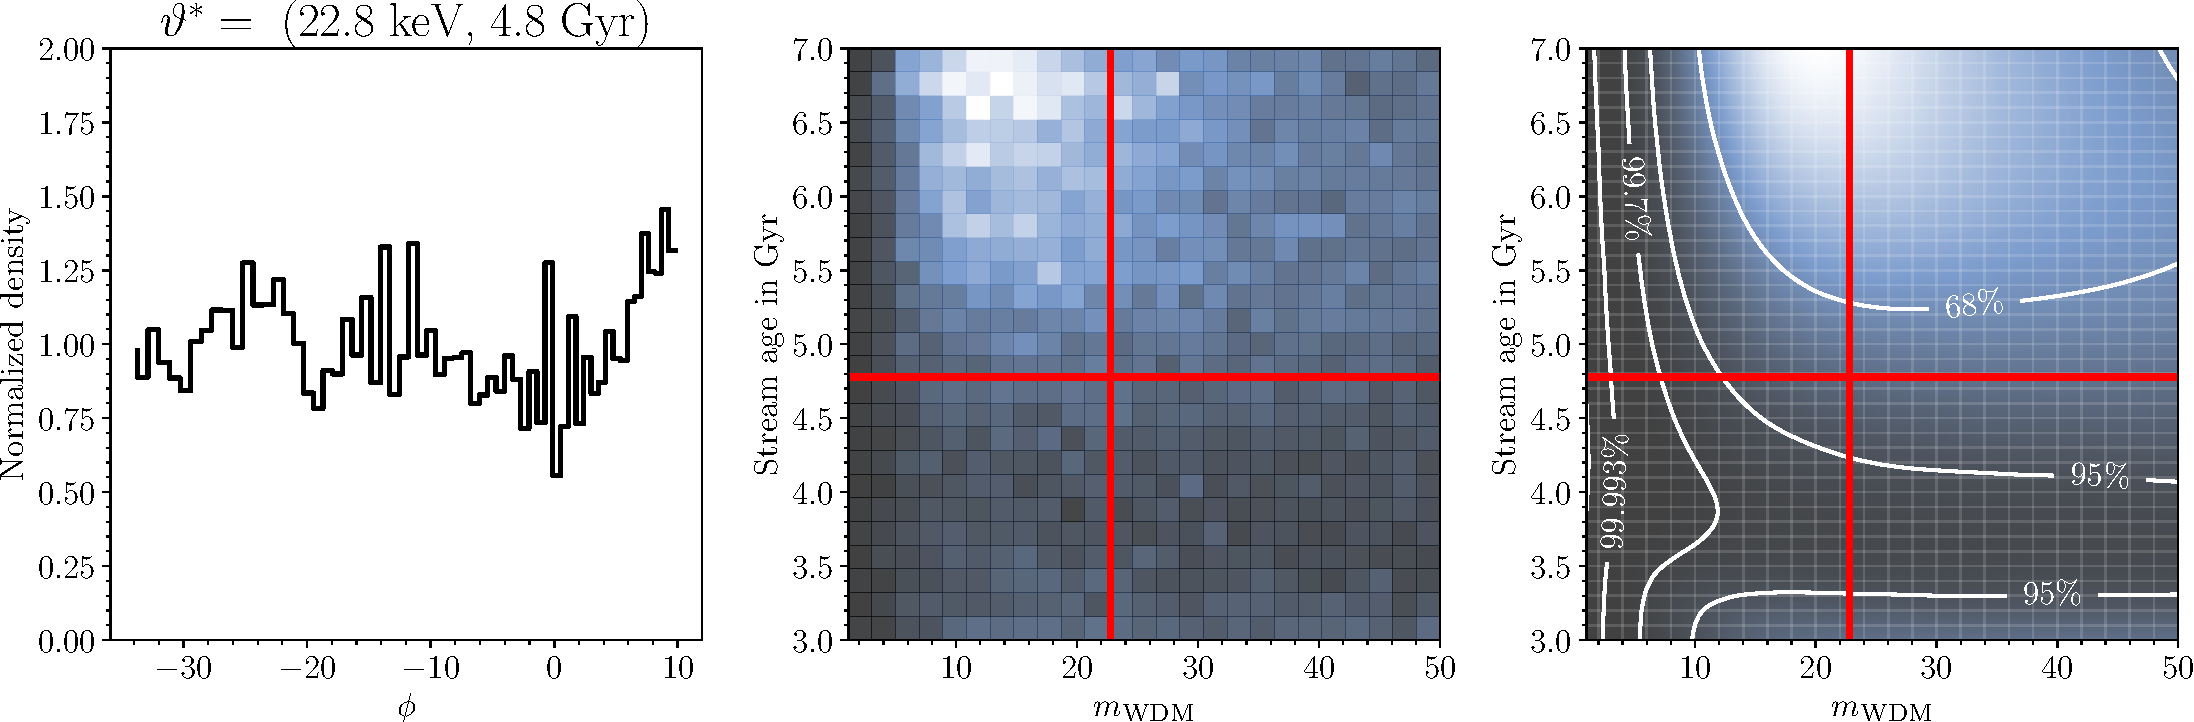
\includegraphics[width=.8\linewidth]{figures/abc-results-compact-combined-horizontal}
    \caption{The columns show, from left to right,
    the observable, the approximate ABC posterior and our method respectively. The red cross indicates the groundtruth.
    ~~\protect\code{https://github.com/JoeriHermans/constraining-dark-matter-with-stellar-streams-and-ml/blob/master/experiments/experiment-inference/out/summary-abc-new.ipynb}}
    %https://github.com/JoeriHermans/constraining-dark-matter-with-stellar-streams-and-ml/experiments/experiments-inference/out/summary-abc-new-comparison.ipynb}}
    \label{fig:abc_results_compact}
\end{figure*}
%No exhaustive hyperparameter optimization or architecture-search was conducted.

\noindent{\bf Approximate Bayesian Computation}~~
Our experimental trials with ABC consider
$s(x) = \mathbb{V}\left[x / x_o\right]$
as a summary statistic, where $x_o$ is the observable of interest.
Given that every observable has a fixed number of bins, we can divide the synthetic observable $x$
by the observable of interest $x_o$. Ideally, if the observables match perfectly, then the
variance of the stellar density ratios is 0.

\subsection{Statistical quality}
\label{sec:diagnostics}
Before making any scientific conclusion, it
is crucial to verify the result of the involved statistical computation.
This is especially challenging in the likelihood-free setting because
the likelihood model is per definition intractable.
The amortization of the ratio estimators enables us to quickly
approximate the posterior of any observable $x$ supported
by the marginal model $p(x)$. It is therefore computationally viable
to assess the quality of the approximation
by determining whether the empirical \emph{coverage}
probability corresponds to the desired confidence level.
In every trial, we evaluate the interval construction on 10,000 unseen observables.
This is repeated 10 times to build up a robust statistic.
The empirical coverage probability of a ratio estimator is therefore based
on approximately 100,000 unseen observables in total.
Although credible regions do not necessarily have a frequentist interpretation, they
closely approximate the nominal coverage probability.
All architectures exhibit similar performance, the \textsc{resnet-50} architecture yields $0.675\pm 0.006$, $0.944\pm 0.002$, $0.996\pm 0.001$ for the confidence levels 0.68, 0.95 and 0.997 respectively~~\protect\code{
https://github.com/JoeriHermans/constraining-dark-matter-with-stellar-streams-and-ml/blob/master/experiments/experiment-inference/out/summary-coverage.ipynb
}. The bias of the ratio estimator is probed by assessing the convergence of the mode towards the nominal target parameters for 1000 independent and identically distributed observables. Figure~\ref{fig:diagnostic_map_convergence} demonstrates a single trial.
\begin{figure*}
    \centering
    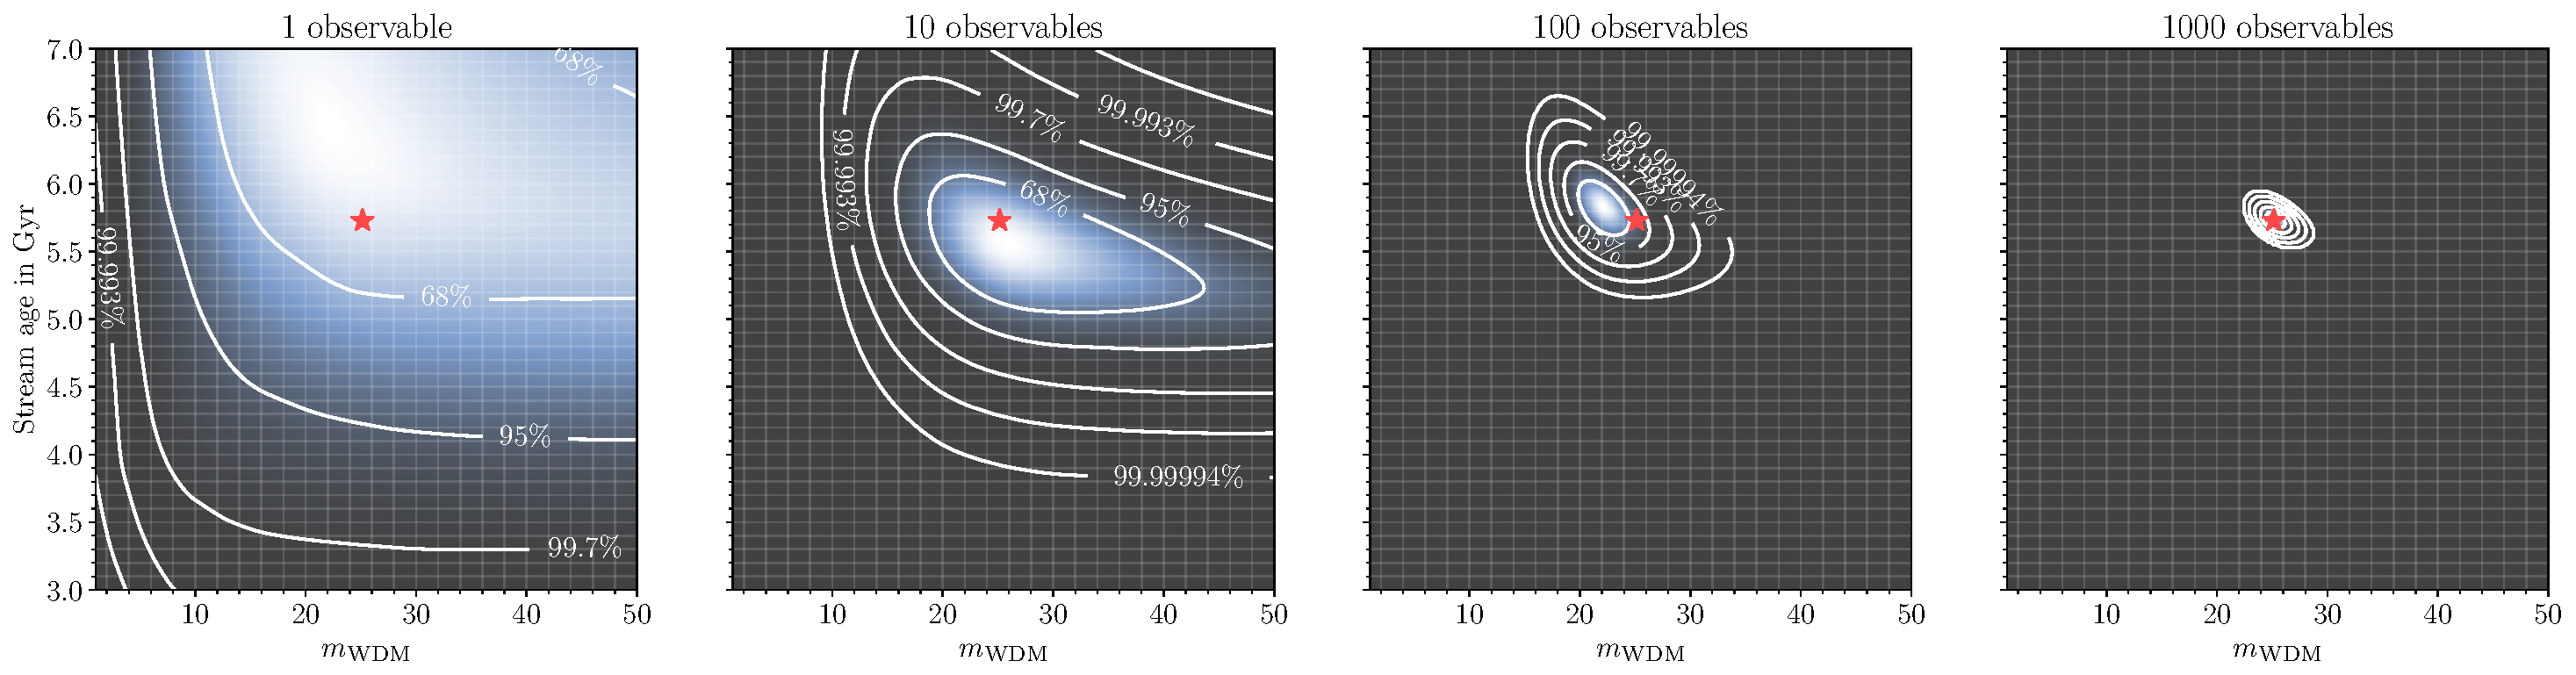
\includegraphics[width=\linewidth]{figures/diagnostic_map_convergence.pdf}
    \caption{Demonstration of the bias probe.
      The figures show, from left to right, the posteriors for 1, 10, 100 and 1000 independent and identically
      distributed mock GD-1 observables.
      As the number of observables increases,
      the posteriors are becoming increasingly more tight around the nominal value.
      This indicates that the posteriors do not, in expectation, introduce signficant bias.
      ~~\protect\code{https://github.com/JoeriHermans/constraining-dark-matter-with-stellar-streams-and-ml/blob/master/experiments/experiment-inference/out/diagnostic-map-convergence.ipynb}}
    \label{fig:diagnostic_map_convergence}
\end{figure*}

\subsection{Direct comparison against ABC}
We find that the structure of the posteriors are, for most mock simulations, in strong agreement.
However, we observe that in some cases our ABC results depend strongly on the adopted summary statistics. 
This highlights the difficulty in
manually constructing an effective summary statistic for high-dimensional data, while this aspect is
completely automated in our approach.
Diagnostics based on (approximate) posterior samples exist~\citep{sbc},
but are not computationally
viable because the posteriors have to be numerically approximated for every test-observable.
Our method does not suffer from this issue, because the estimation of the
posterior density is amortized.
%OLD
%We find that the structure of the posteriors are, for most mock simulations, in strong agreement.
%Cases exists where ABC fails to recover the nominal target parameters, while
%the maximum a posteriori of the proposed methodology concurs with the groundtruth.
%This result, in conjunction with the aforegoing statistical validation of the ratio estimators,
%suggests that the summary statistic is not sufficient. At the same time, this highlights the difficulty in
%manually constructing an effective summary statistic for high-dimensional data, while this aspect is
%completely automated in our approach.
%Diagnostics based on (approximate) posterior samples exist~\citep{sbc},
%but are not computationally
%viable because the posteriors have to be numerically approximated for every test-observable.
%Our method does not suffer from this issue, because the estimation of the
%posterior density is amortized.
% OLD
%
%Interestingly, the posteriors computed by \textsc{abc-a} and \textsc{abc-b} are significantly distinct.
%The structure of the posteriors in \textsc{abc-b}
%and our method are on the other hand, for most mock simulations, in strong agreement.
%Both \textsc{abc} analyses fail to
%recover the nominal target parameter at $\vartheta^*\triangleq$ (7 Gyr, 50 keV), while
%the maximum a posteriori of the proposed methodology concurs with the groundtruth.
%We hypothesize the \textsc{abc} analyses compute this particular approximation
%due to the low power of the density variations in the simulated mock stream,
%which is supported by the fact that the majority of the low $m_\textsc{wdm}$ realizations
%exhibit smaller density variations.
%This result, in conjunction with the aforegoing statistical validation of the ratio estimators,
%forces us to question the necessary sufficiency of the summary statistics.
%Diagnostics based on (approximate) posterior samples exist~\citep{sbc},
%but are not computationally
%viable because the posteriors have to be numerically approximated for every test-observable.
%Our method does not suffer from this issue, because the estimation of the
%posterior density is amortized. In addition, the comparisons suggest the proposed
%methodology is more sensitive to high keV realisations.
\begin{figure*}[!b]
    \centering
    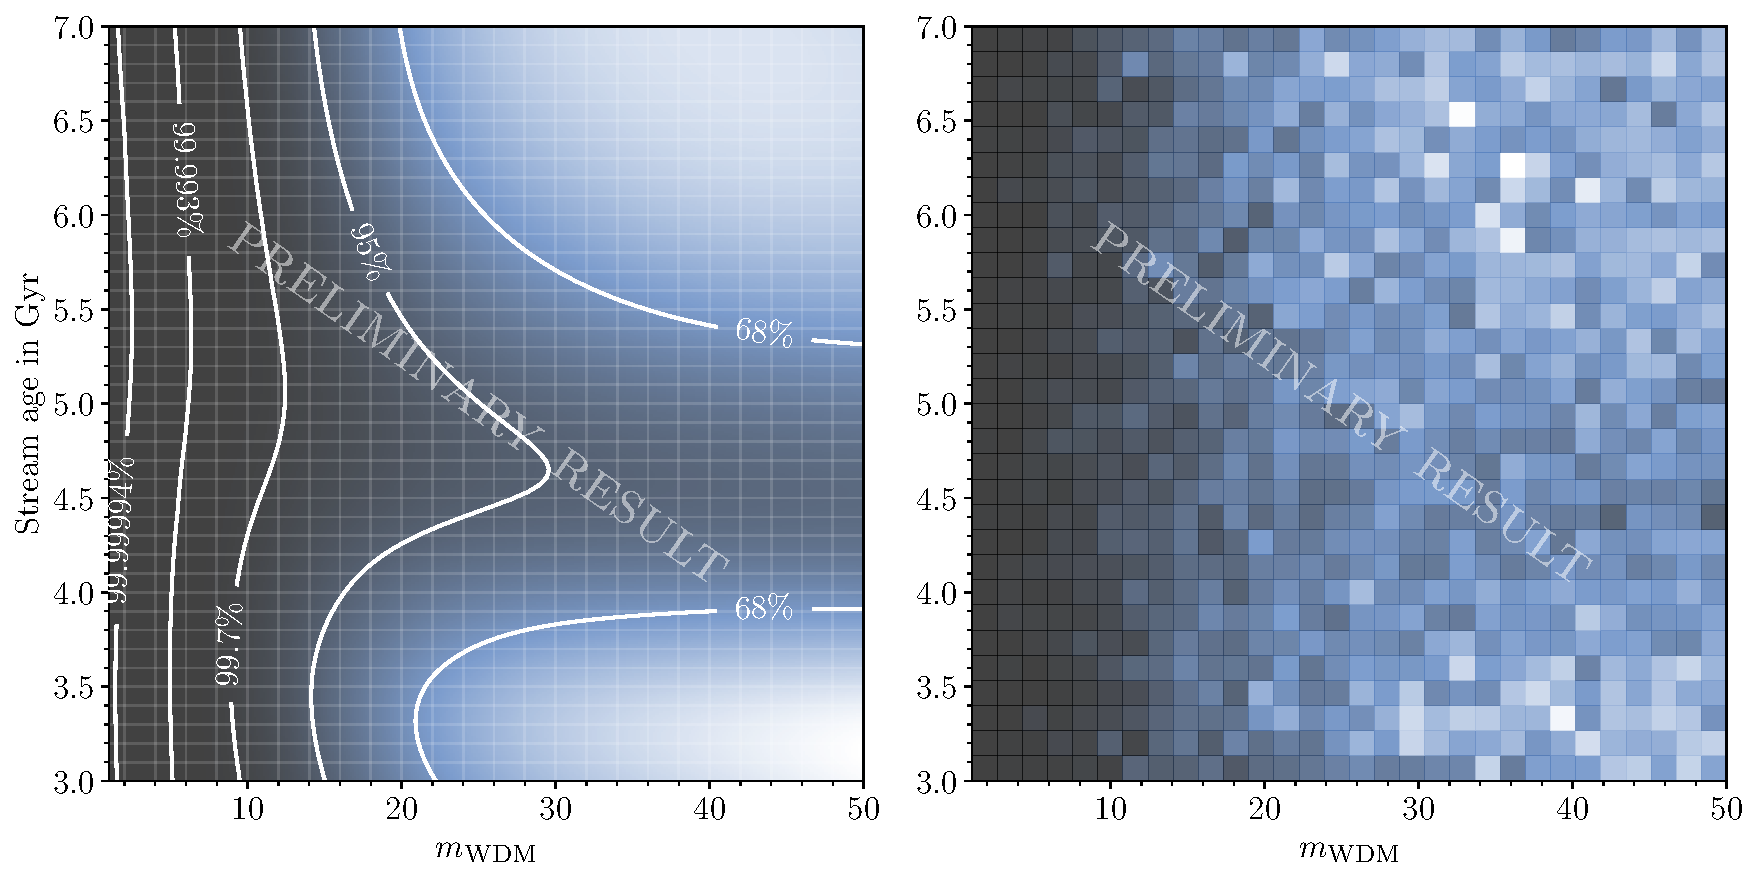
\includegraphics[width=.8\linewidth]{figures/posterior-gd1-all-2d}
    % 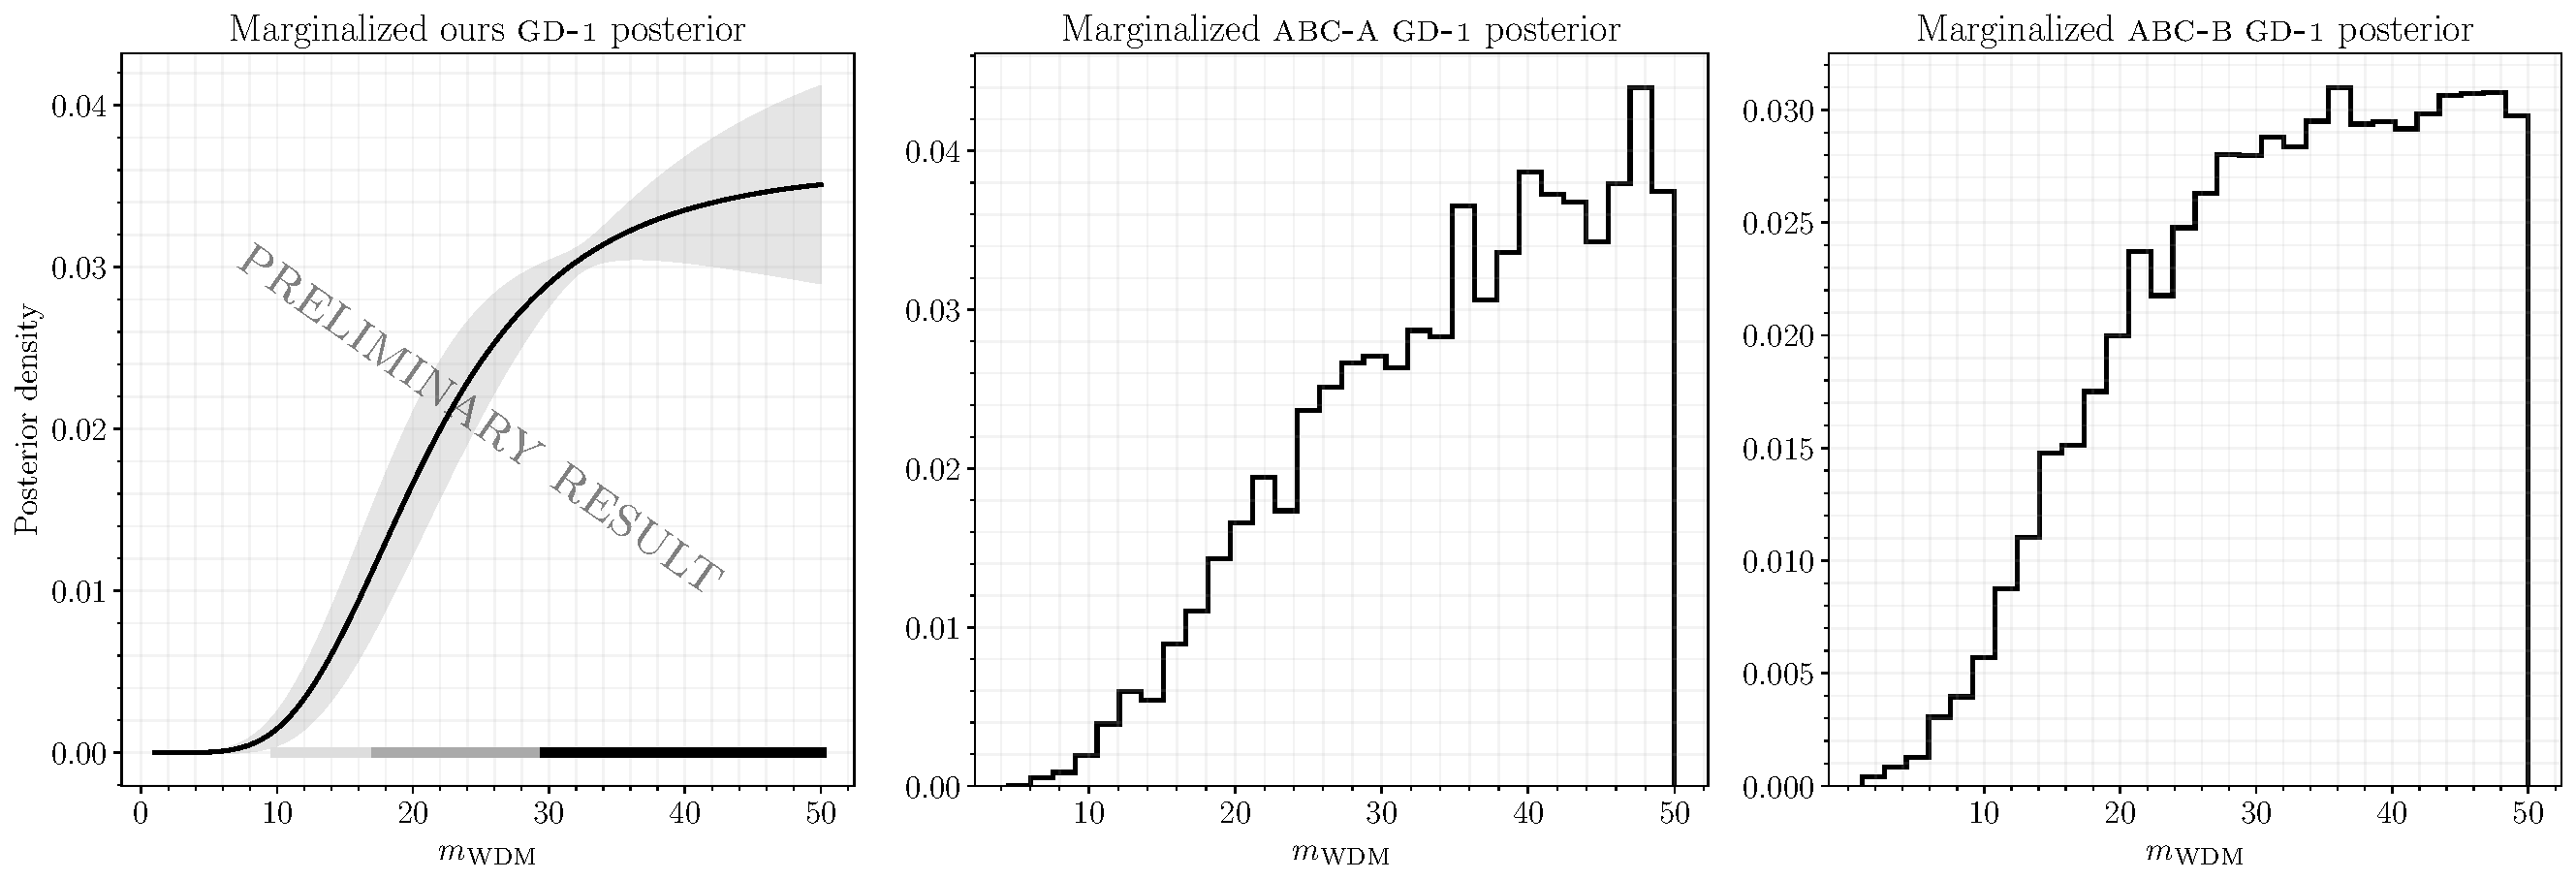
\includegraphics[width=\linewidth]{figures/posterior-gd1-all-1d}
    \caption{Posteriors based on the observed stellar density variations of GD-1.
    The figure shows, from left to right, our method and ABC respectively.
    The constraints are based on credible regions. All posteriors indicate a preference for CDM over WDM within the assumed simulation model.
    ~~\protect\code{https://github.com/JoeriHermans/constraining-dark-matter-with-stellar-streams-and-ml/blob/master/experiments/experiment-inference/out/summary-gd1-inference.ipynb}}
    \label{fig:gd1_posteriors}
\end{figure*}

\subsection{Preliminary constraints on $m_\textsc{wdm}$ using data on GD-1}
We compute \emph{preliminary} constraints on $m_\textsc{wdm}$
based on
the observed stellar density along the GD-1 stream which was obtained using \emph{Gaia} proper motions~\citep{gaia,2016A&A...595A...1G}
and \emph{Pan-STARRS} photometry~\citep{2017AAS...22922303C}.
We stress that {\bf our simulation model does not account for baryonic effects, disturbances caused by massive ($> 10^9~\Msun$) subhalos, and effects induced by variations in the Milky Way potential.}
%and hence our constraints only hold under the assumed simulation model.
The posteriors and corresponding credible regions are shown in Figure~\ref{fig:gd1_posteriors}.
In this context, all independent analyses have a strong preference for CDM over WDM.
After marginalizing the stream age, the proposed methodology yields $m_\textsc{wdm}\geq 17.5$ keV (95\% \textsc{cr}) and $m_\textsc{wdm}\geq 10.5$ keV (99.7\% \textsc{cr}). 
Assuming the posterior approximated by ABC is exact, we find 
$m_\textsc{wdm}\geq 10.2$ keV (95\% \textsc{cr}) and $m_\textsc{wdm}\geq 5.0$ keV (99.7\% \textsc{cr}).
Our results are promising and indicate that with the proposed method we could effectively exclude the  sterile neutrino~\cite{dodelson1994sterile,shi1999new,abazajian2001sterile,asaka2005numsm,boyarsky2009role} as a possible candidate for the dark matter particle, provided simulator systematics can be brought under control.

%.  The urgent next step is to reassess and improve all simulator systematics, for which 
%baryonic effects and other simulator systematics can be fully accounted for in future analysis.

\section*{Broader impact}
The approach could provoke a shift in the way likelihood-free statistical inference is done in the physical sciences.
Previous approaches, such as Approximate Bayesian Computation, require a handcrafted sufficient summary statistic and distance metric.
The specific definition of both components can significantly influence the approximated posteriors. Instead, our approach automatically \emph{learns} an efficient internal representation of the
relation between the model parameters and the observables, and therefore permits domain-scientits to pivot
from attempting to solve the interactable inverse problem --- by defining \emph{assumed} sufficient summary statistics --- to the more natural forward modelling of the phenomena of interest.
The machine learning component would thus handle the inference aspect.
Finally, the amortization of the posterior estimates enables thorough statistical validation of the neural networks to ensure qualitative posteriors.
Something which is not feasible in ABC analyses.


\begin{ack}
  Joeri Hermans would like to thank the National Fund for Scientific Research for his FRIA scholarship.
  Gilles Louppe is recipient of the ULiège - NRB Chair on Big data and is thankful for the support of NRB.
  All authors would like to thank the developers of the \emph{Jupyter}~\citep{jupyter} project, \emph{Matplotlib}~\citep{matplotlib},
  \emph{Numpy}~\citep{numpy}, \emph{PyTorch}~\citep{paszke2017automatic},
  and \emph{Scikit-Learn}~\citep{scikit-learn} for enabling this work.
\end{ack}

\bibliographystyle{unsrtnat}
\bibliography{main}

\end{document}